%************************************************
\chapter{Mobile visual assistive apps: a description of the problem and motivation}\label{ch:chapter2}
%************************************************

\section{Introduction}

Although the use of computer vision to analyse images from smartphones and wearable cameras is in its infancy, the opportunity to exploit these devices for various assistive applications is beginning to emerge. In this chapter, two potential applications of computer vision in the assistive context for blind and partially sighted users are considered. These two applications are intended to help provide answers to the questions posed in Chapter~\ref{ch:introduction}: ``Where am I?'' and ``What am I holding?''.

Taking into account the context of mobile devices and assistive applications, I present the motivation to study appearance-based methods for indoor localisation and object recognition, and describe two pilot studies that lay the foundations for the work described in subsequent chapters:

\begin{itemize}
\item First, it is possible to suggest how to go about providing estimates of the indoor location of a user through queries submitted by a smartphone camera against a database of \textit{visual paths} -- descriptions of the visual appearance of common journeys that might be taken with a hand-held or wearable device. My proposal is that such journeys could be harvested from, for example, sighted volunteers. Initial tests using bootstrap statistics do indeed suggest that there is sufficient information within such visual path data to provide indications of: a) along which of several routes a user might be navigating; b) where along a particular path they might be.
\item The second pilot presented in this chapter is a study of the need for a new benchmarking database and test set for answering the second question of ``What am I holding?''. The database acquisition and evaluation experiments will be discussed in detail in Chapter \ref{ch:chapter3}, however in this chapter I will discuss the requirements that are needed for specific mobile context and assistive applications.
\end{itemize}



%% WHERE AM I?

\section{Where Am I?}

Techniques for WiFi localisation are entering mainstream use through, at one level, estimates obtained from the physical locations of WiFi access points, simple measures of signal strength or approaches such as ``Walkie-Markie''~\cite{Shen}, which use mul\-ti\-ple\--sensor signatures to infer location.  These technologies hold great potential.  However, accurate localisation still relies strongly on reasonable accurate motion models, and the collection of other cues, such as accelerometry or gyroscopes \cite{Wang2012}.  

Indeed, no matter how good other sources of information are, few can replace the contextual information of visual inference.  During navigation, using natural vision, sighted individuals are able to {\em from one consistent information source}: a) recognise their location relative to previous journeys; b) locate entrances and exits; c) detect obstructions; d) recognise people; e) assess human intent;
f) identify objects or activities of personal interest.

Invoking computer vision to \textit{simultaneously} solve all of these tasks is a current challenge.  The purpose of the initial work reported in this chapter is to assess the feasibility and accuracy of existing computer vision techniques to meet some of these needs.  The primary question addressed in this section relates to the first topic in the list above: can we use computer vision to recognise locations against previous journeys?

\subsection{Related Approaches}
 
In Chapters \ref{ch:chapter4}, \ref{ch:chapter5} and \ref{ch:chapter6} a more detailed collection of related methods for indoor localisation is provided with emphasis in the specific context of each chapter. In all of them there are references to simultaneous localisation and mapping (SLAM \cite{Durrant-Whyte2006}) and parallel tracking and mapping (PTAM, \cite{klein2009parallel}) as these and derived approaches are the techniques that  are near state-of-the-art for monocular robot navigation, allowing geometry of a space to be mapped out dynamically at the same time that self-localisation is achieved.  In the assistive context, Pradeep and colleagues successfully applied this to a demonstration for indoor navigation in an assistive device \cite{Pradeep2010}.

Several methods of indoor localisation using smartphone\--re\-le\-vant technology have also been the object of study, including RSSI, dead-reckoning, and combinations of techniques that harvest environmental cues \cite{Wang2012,Shen}. 
 

\subsection{Visual Paths} 

 As we will see later in more detail in Chapter \ref{ch:chapter4}, methods such as SLAM and PTAM attempt to simultaneously map world geometry and localise a camera within that geometry.  The question here is slightly different: we seek to identify where one might be relative to previous journeys taken along the same route, either by ourselves or other people.  Thus, I introduce the idea of the \textit{visual path}, a stream of descriptions captured from visual information as we traverse from location $A$ to location $B$, or from location $C$ to $D$. Such streams could be captured from the cameras of other users moving in the same physical space.

The path localisation problem can be split into two distinct tasks.  The first is to determine which of $P$ possible paths one is navigating along, and the second is to determine where along a particular visual path one is located.  In the context of computer vision, a key question concerns the \textit{distinctiveness} of information along paths, either as indicators of a particular journey or as indicators of location along a known journey.  Note that localisation with respect to a map is not explicitly attempted -- the suggestion is to localise with respect to a journey.  In the context of many users, this would appear to be a sensible way to harvest information about locations that might be frequently reconfigured in a manner that would reduce dependence on explicit mapping processes.

Though SLAM and PTAM are strong candidates for assistive techniques, there is also the need to combine mapping with object detection and other types of semantic information.  Putting these systems in the category of mapping and localisation, I explore the possibility that rather than mapping out a space, a user might be more interested in merely following a path that has been traversed by others.  It is in this long-term, collaborative context that the visual path concept would sit: we wish to allow users to compare their journeys against those of others through these visual paths (see Figure \ref{fig:associatingViews}).

\begin{figure}[h]
\centering
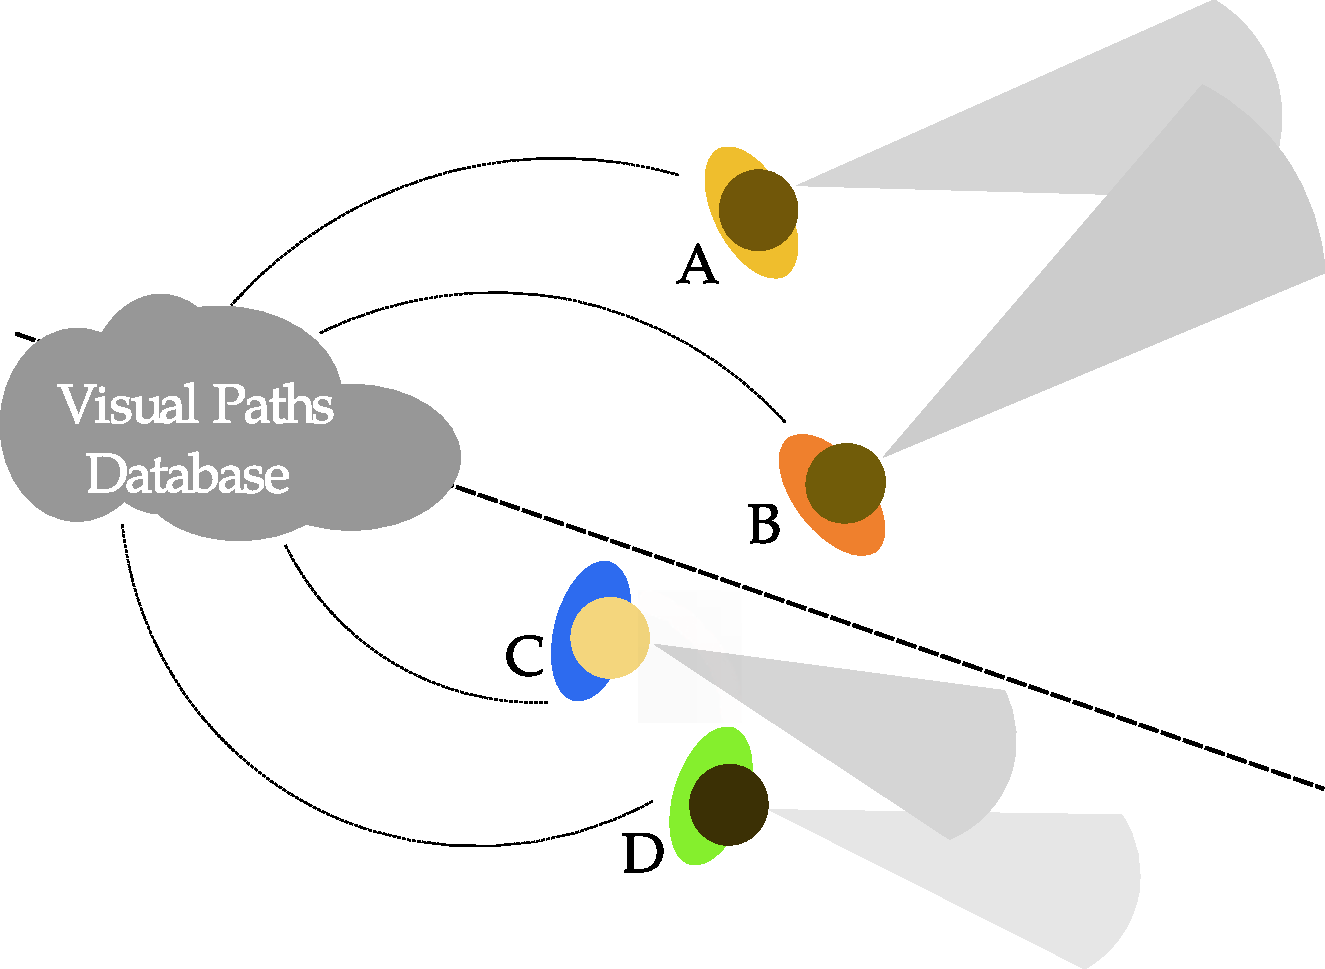
\includegraphics[width=0.8\textwidth]{./gfx/Chapter02/AssociatingViews.pdf}
\caption{Crowdsourcing indoor journeys (``visual paths'') from multiple users.  Users $A$ and $B$ make the same journey at different points in time, but can associate their journeys through storing their visual paths on a server; other users $C$ and $D$, make different journeys, but again can associate their experiences with each other. The statistical tests reported in this chapter compare the within-path queries and between-path queries, as well as within-path, between-location scores based on image comparisons.}
\label{fig:associatingViews}
\end{figure}

In tracing along different paths, one might ask how distinctive the visual content is along one path relative to the appearance along another. In this pilot study I used a standard keypoint and descriptor type approaches -- the SIFT keypoint and descriptor -- to describe visual paths captured by users as they walked along indoor environments. The same type of image description will be subject of a dedicated study in Chapter \ref{ch:chapter4}.

I first studied the distribution of a similarity metric, $\gamma$, based on a modification of Lowe's ratio test for discriminating descriptors~\cite{lowe2004distinctive}. The modification takes the form of an $L_{\infty}$-type normalisation on the distribution of squared Euclidean distances between distinctive descriptors that are close matches between database images along a set of $P$ possible paths $C_p,\,p=1,2,\ldots, P$.

For the preliminary work described in this chapter, \textit{sparse}\footnote{Also known as keypoint-based SIFT, or more frequently, just SIFT.} SIFT descriptors are used. For a detailed description of how these descriptors, or feature vectors, are computed, refer to Chapter \ref{ch:chapter4}.


\subsection{Visual Path Descriptions} First, consider a number $M_p^{(i)}$ of descriptor vectors, $\mathbf{v}_m^{(i)}, m=1,2,\ldots,M^{(i)}$ produced from an image, $\mathbf{I}^{(i)}_p$, with each vector being of  dimension $L \times 1$.  These descriptors are stacked into the rows of an $M^{(i)}\times L$ descriptor matrix, $\mathbf{V}^{(i)}_p$ associated with image $\mathbf{I}^{(i)}_p$.  A \textit{set} of images, $\lbrace \mathbf{I}^{(i)}_p\rbrace_{i=1,2,\ldots\,N_p}$ is now collected for path $C_p$, and for each of these, a descriptor matrix is produced.  A visual path $C_p$ is then encoded by the set of matrices of descriptors, denoted $\mathcal{M}_p=\lbrace \mathbf{V}^{(i)}_p \rbrace_{i=1,2,\ldots,N_p}$ generated from the set of images taken along that path.
 
Query images, $\mathbf{J}^{(j)}$, $j=1,2,\ldots,N_q$ are now acquired, separately.  A particular query image is also mapped to matrix of descriptors $\mathbf{Q}^{(j)}$. We wish to know which of the $P$ paths the query image $\mathbf{J}^{(j)}$ has been taken on; this is answered by comparing the query descriptor matrix against the set of path descriptors for all paths, $\lbrace \mathcal{M}_p \rbrace_{p=1,2,\ldots, P}$.

\subsection{Pairwise Descriptor Comparisons} \label{subsec:pairwise}

Let us first consider the comparison of individual query descriptors, $\mathbf{v}_n^{(j)}, n=1,2,\ldots,N^{(j)}$ arising from a single query image.  The Euclidean distance metric in $L$-dimensional space is widely used in assessing descriptor distances in computer vision.  Let $\mathbf{D}^{(i|n)}$ be the $M^{(i)}\times L$ matrix defined by

\begin{equation}
\centering
\mathbf{D}^{(i|n)}_p =  \mathds{1}_{M^{(i)}\times 1} \otimes \mathbf{v}_n^{(j)} - \mathbf{V}^{(i)}_p,
\end{equation}

where $\mathds{1}$ is a vector of ones, and $\otimes$ denotes the Kronecker product.
Then, the elements along the diagonal of

\begin{equation}
\centering
 \mathbf{D}^{(i|n)}_p[\mathbf{D}^{(i|n)}_p]^T,
\end{equation}

are collated into a vector, $\mathbf{d}^{(i|n)}_p \in [0,\mathbb{R}^+]^{M^{(i)}}$ of squared Euclidean distances between the $n^{th}$ descriptor from a query image and each of the $M^{(i)}$ descriptors derived from the $i^{th}$ image along the path $C_p$. 

\subsection{Query Descriptor Rejection} \label{subsec:querydescrejection}
Many descriptors in the query image will not be sufficiently distinct to be useful in matching.  The distribution of distances contained in vector $\mathbf{d}^{(i|n)}_p$ is used in a first stage filtering for distinctiveness by order-statistic filtering.  A query descriptor $\mathbf{v}_n^{(j)}$ is considered suitable for use in assessing similarity between a pair of images only if $d^{(i|n)}_{[1]} < \alpha \cdot d^{(i|n)}_{[2]}$ where $d^{(i|n)}_{[1]}, d^{(i|n)}_{[2]},\ldots $ denotes the sorted elements of the vector $\mathbf{d}^{(i|n)}_p$ in increasing order (the path subscript $p$ is temporarily suppressed to include the order-statistic of elements).  $0<\alpha<1$ is set to around 0.7, and any \textit{query} descriptors that do not satisfy this condition is discarded. This ``uniqueness criterion'' was chosen by Lowe as the ratio of closest to second-closest neighbours of each descriptor that provides the best ratio of probabilities for correct versus incorrect matches~\cite{lowe2004distinctive}. All image query vectors are subjected to the same test.  Those that pass the test allow an ``average'' distance based on best matching descriptors to be used to determine how close a single query image is to a single database image. That is, for a single image query 

\begin{equation}
\centering
\mu^{(i,j)}_p=\frac{1}{|\mathcal{D}|}\sum_{n\in \mathcal{D}} d^{(i|n)}_{[1]},
\end{equation}

is calculated where $\mathcal{D}$ is the set of query descriptors that pass the distinctiveness test, as described here. Again, note that path subscript $p$ has been omitted from the right-hand side of this expression to represent the sorted distances.

\subsection{The $\gamma$ Score} I calculated  $\mu_p^{(i,j)}$ across all query images $\mathbf{J}^{(j)}$, $j=1,2,\ldots,N_q$ and all path images $\lbrace\lbrace I^{(i)}_p\rbrace_{i=1,2,\ldots,N_p}\rbrace_{p=1,2,\ldots P}$.   A score is then defined to produce a measure of similarity $\gamma^{(i,j)}$ between image pairs $(i,j)$ relative to path $p$ such that $0 < \gamma \le 1$. 


\begin{equation}
\centering
\gamma^{(i,j)} = \frac{||\mu^{(i,j)}_p||_{\infty}-\mu^{(i,j)}_p}{||\mu^{(i,j)}_p||_{\infty}}.
\end{equation}

This score is calculated between pairs of query and database images, and one may identify two types of categories that these query comparisons fall into.  In the first case, the images come from the same path (although query and visual path database are, of course, distinct).  In the other case, queries come from different paths. %The results are shown in Figure~\ref{fig:gammaDistribution} where $f_\gamma$ denotes the probability density distribution (PDF) of the $\gamma$ score and $QC_x$ and $DC_x$ indicate query and database corridor $x$ respectively.   

%\begin{figure}[ht]
%\centering
%{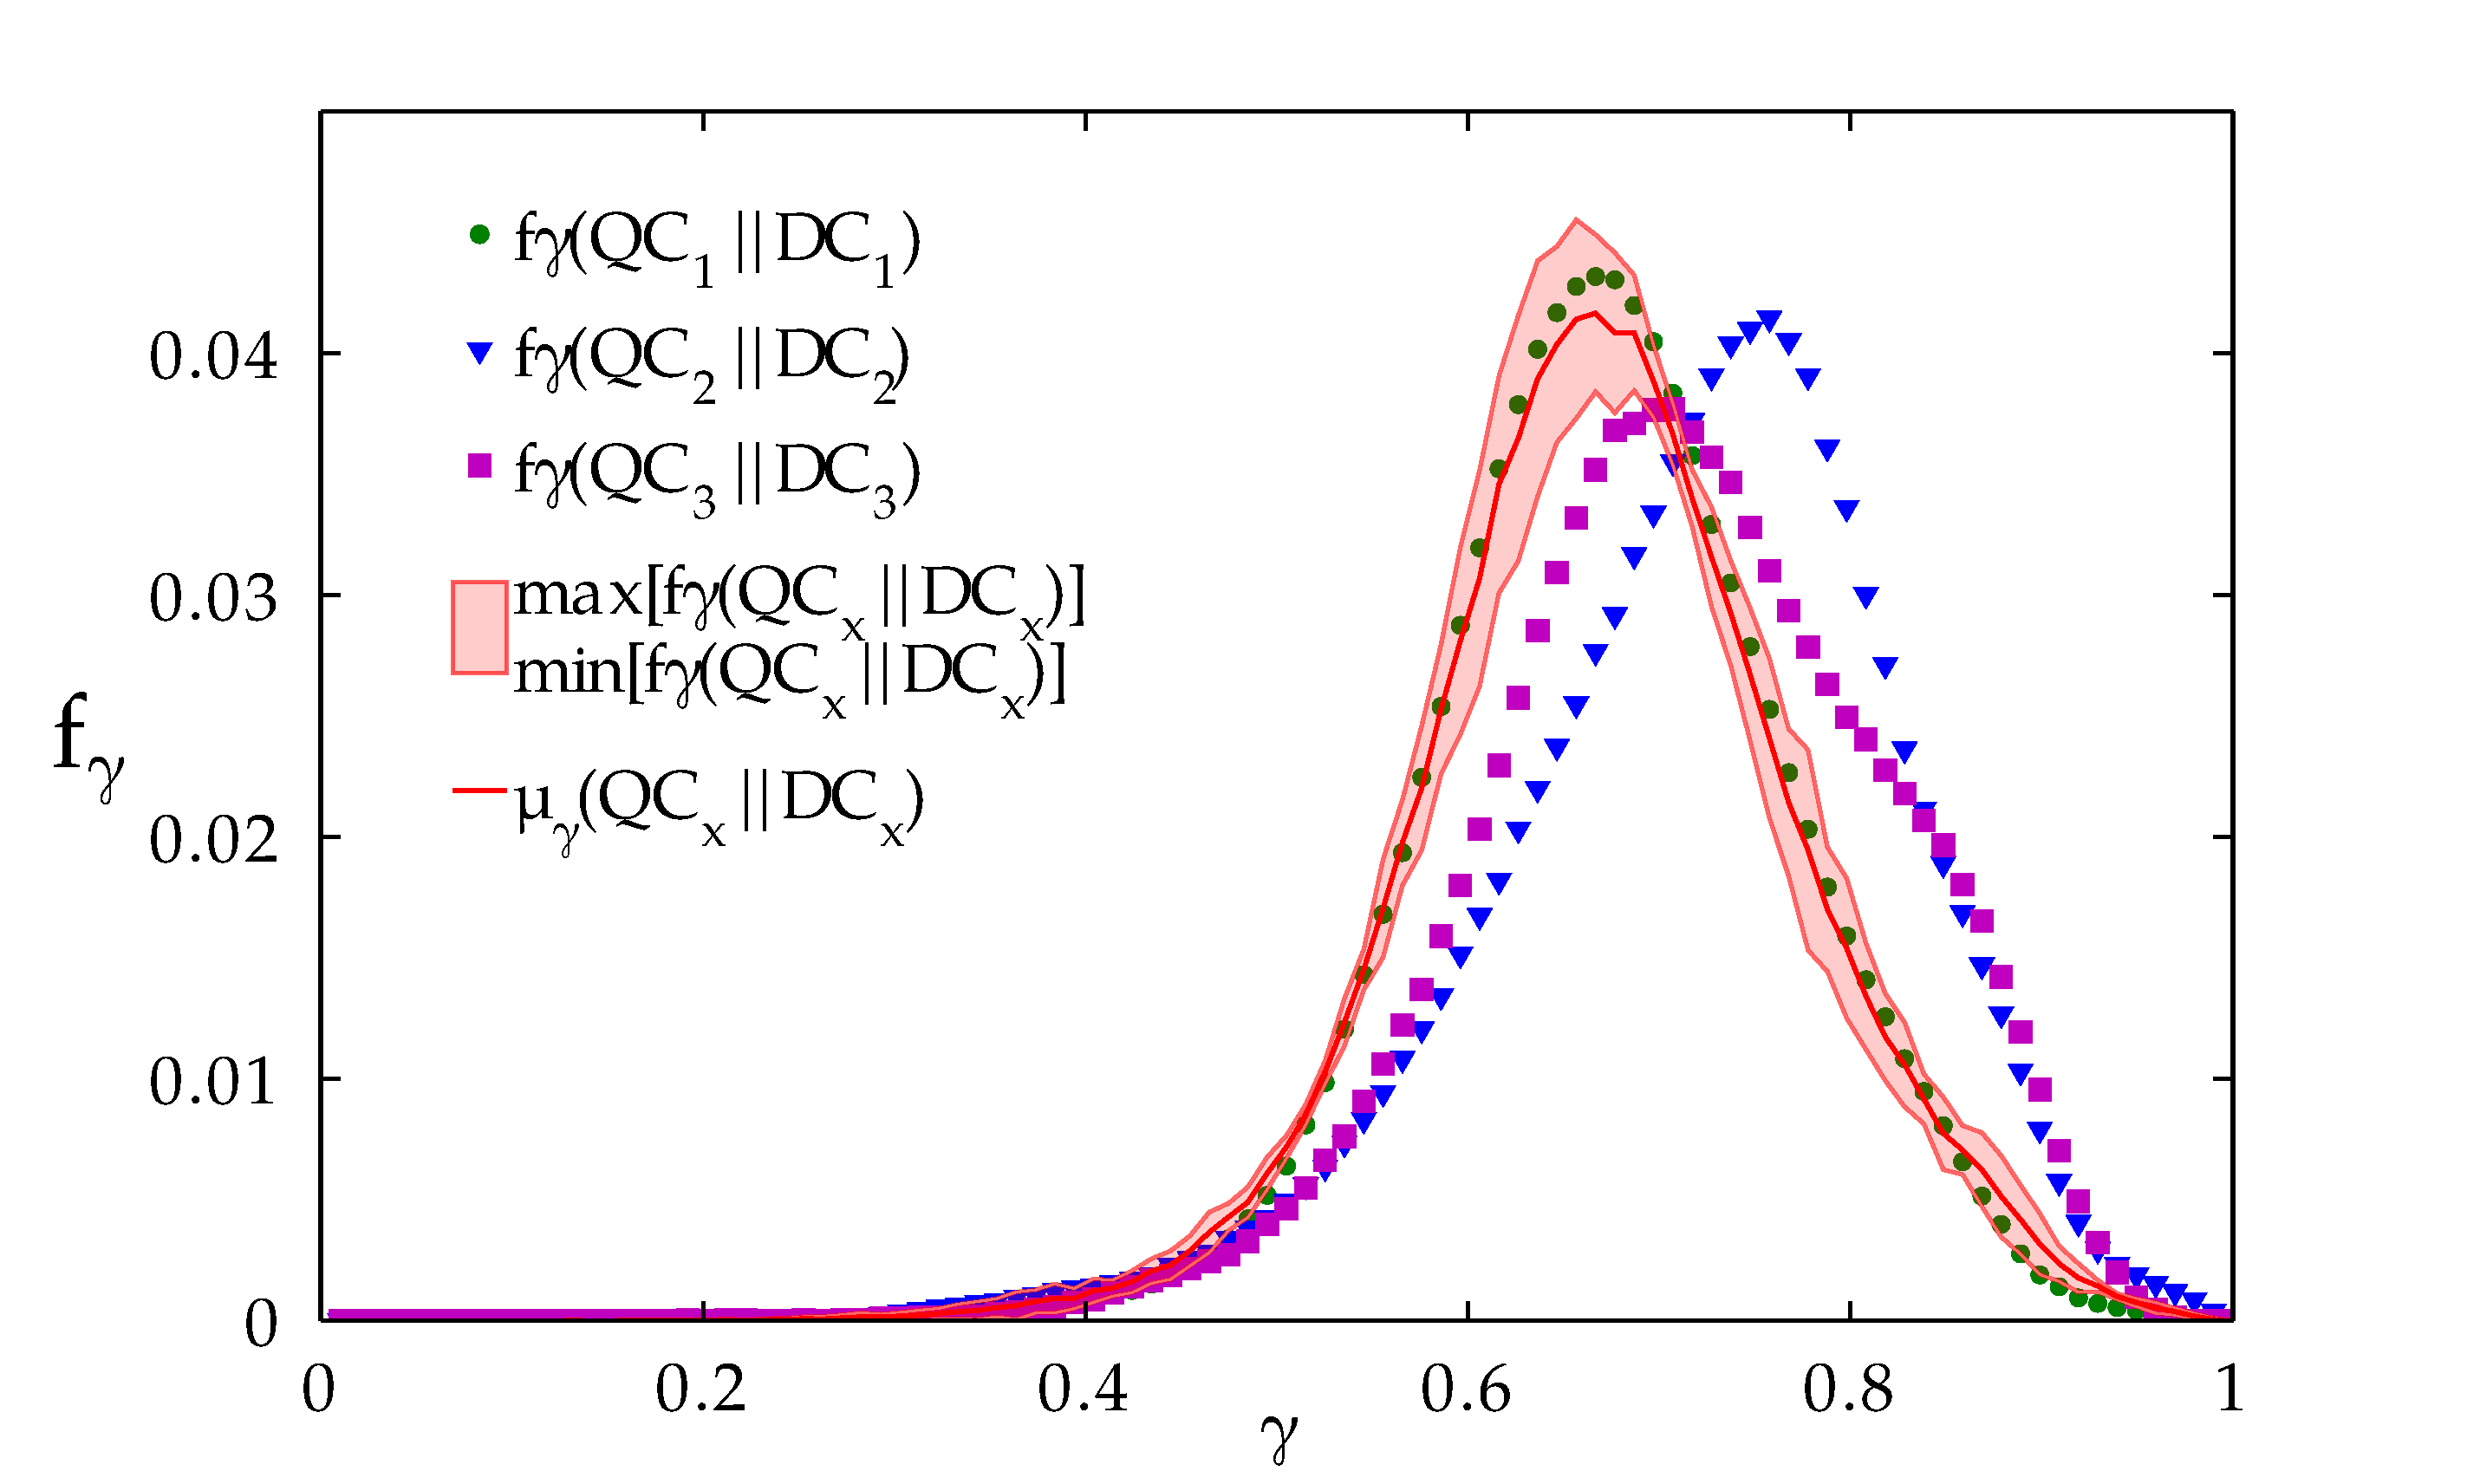
\includegraphics[width=\linewidth]{./gfx/Chapter02/path_pdf_analysisWithShadedBetweensALLDB.pdf}}
%\caption{Tests of visual distinctiveness along paths: Distributions for the $\gamma$ score. Path level queries, capturing the behaviour of the $\gamma$ score for different corridors.}
%\label{fig:gammaDistribution}
%\end{figure}
 



A second type of score, $\rho$, was created with a slightly different normalisation criterion based on observing the maximum within-path distance distributions, i.e. for a given path index, $p$.  The behaviour of this score was studied using query images as taken with ground-truth locations, measured with a surveyor's wheel in preliminary experiments on what it would later be the RSM dataset described in Chapter \ref{ch:chapter4}. Again, probability density estimates of scores are estimated from hundreds of thousands of descriptor comparisons and are represented as $f_\rho$ in Figure~\ref{fig:rhoDistribution}.


\begin{figure}[ht]
\centering
{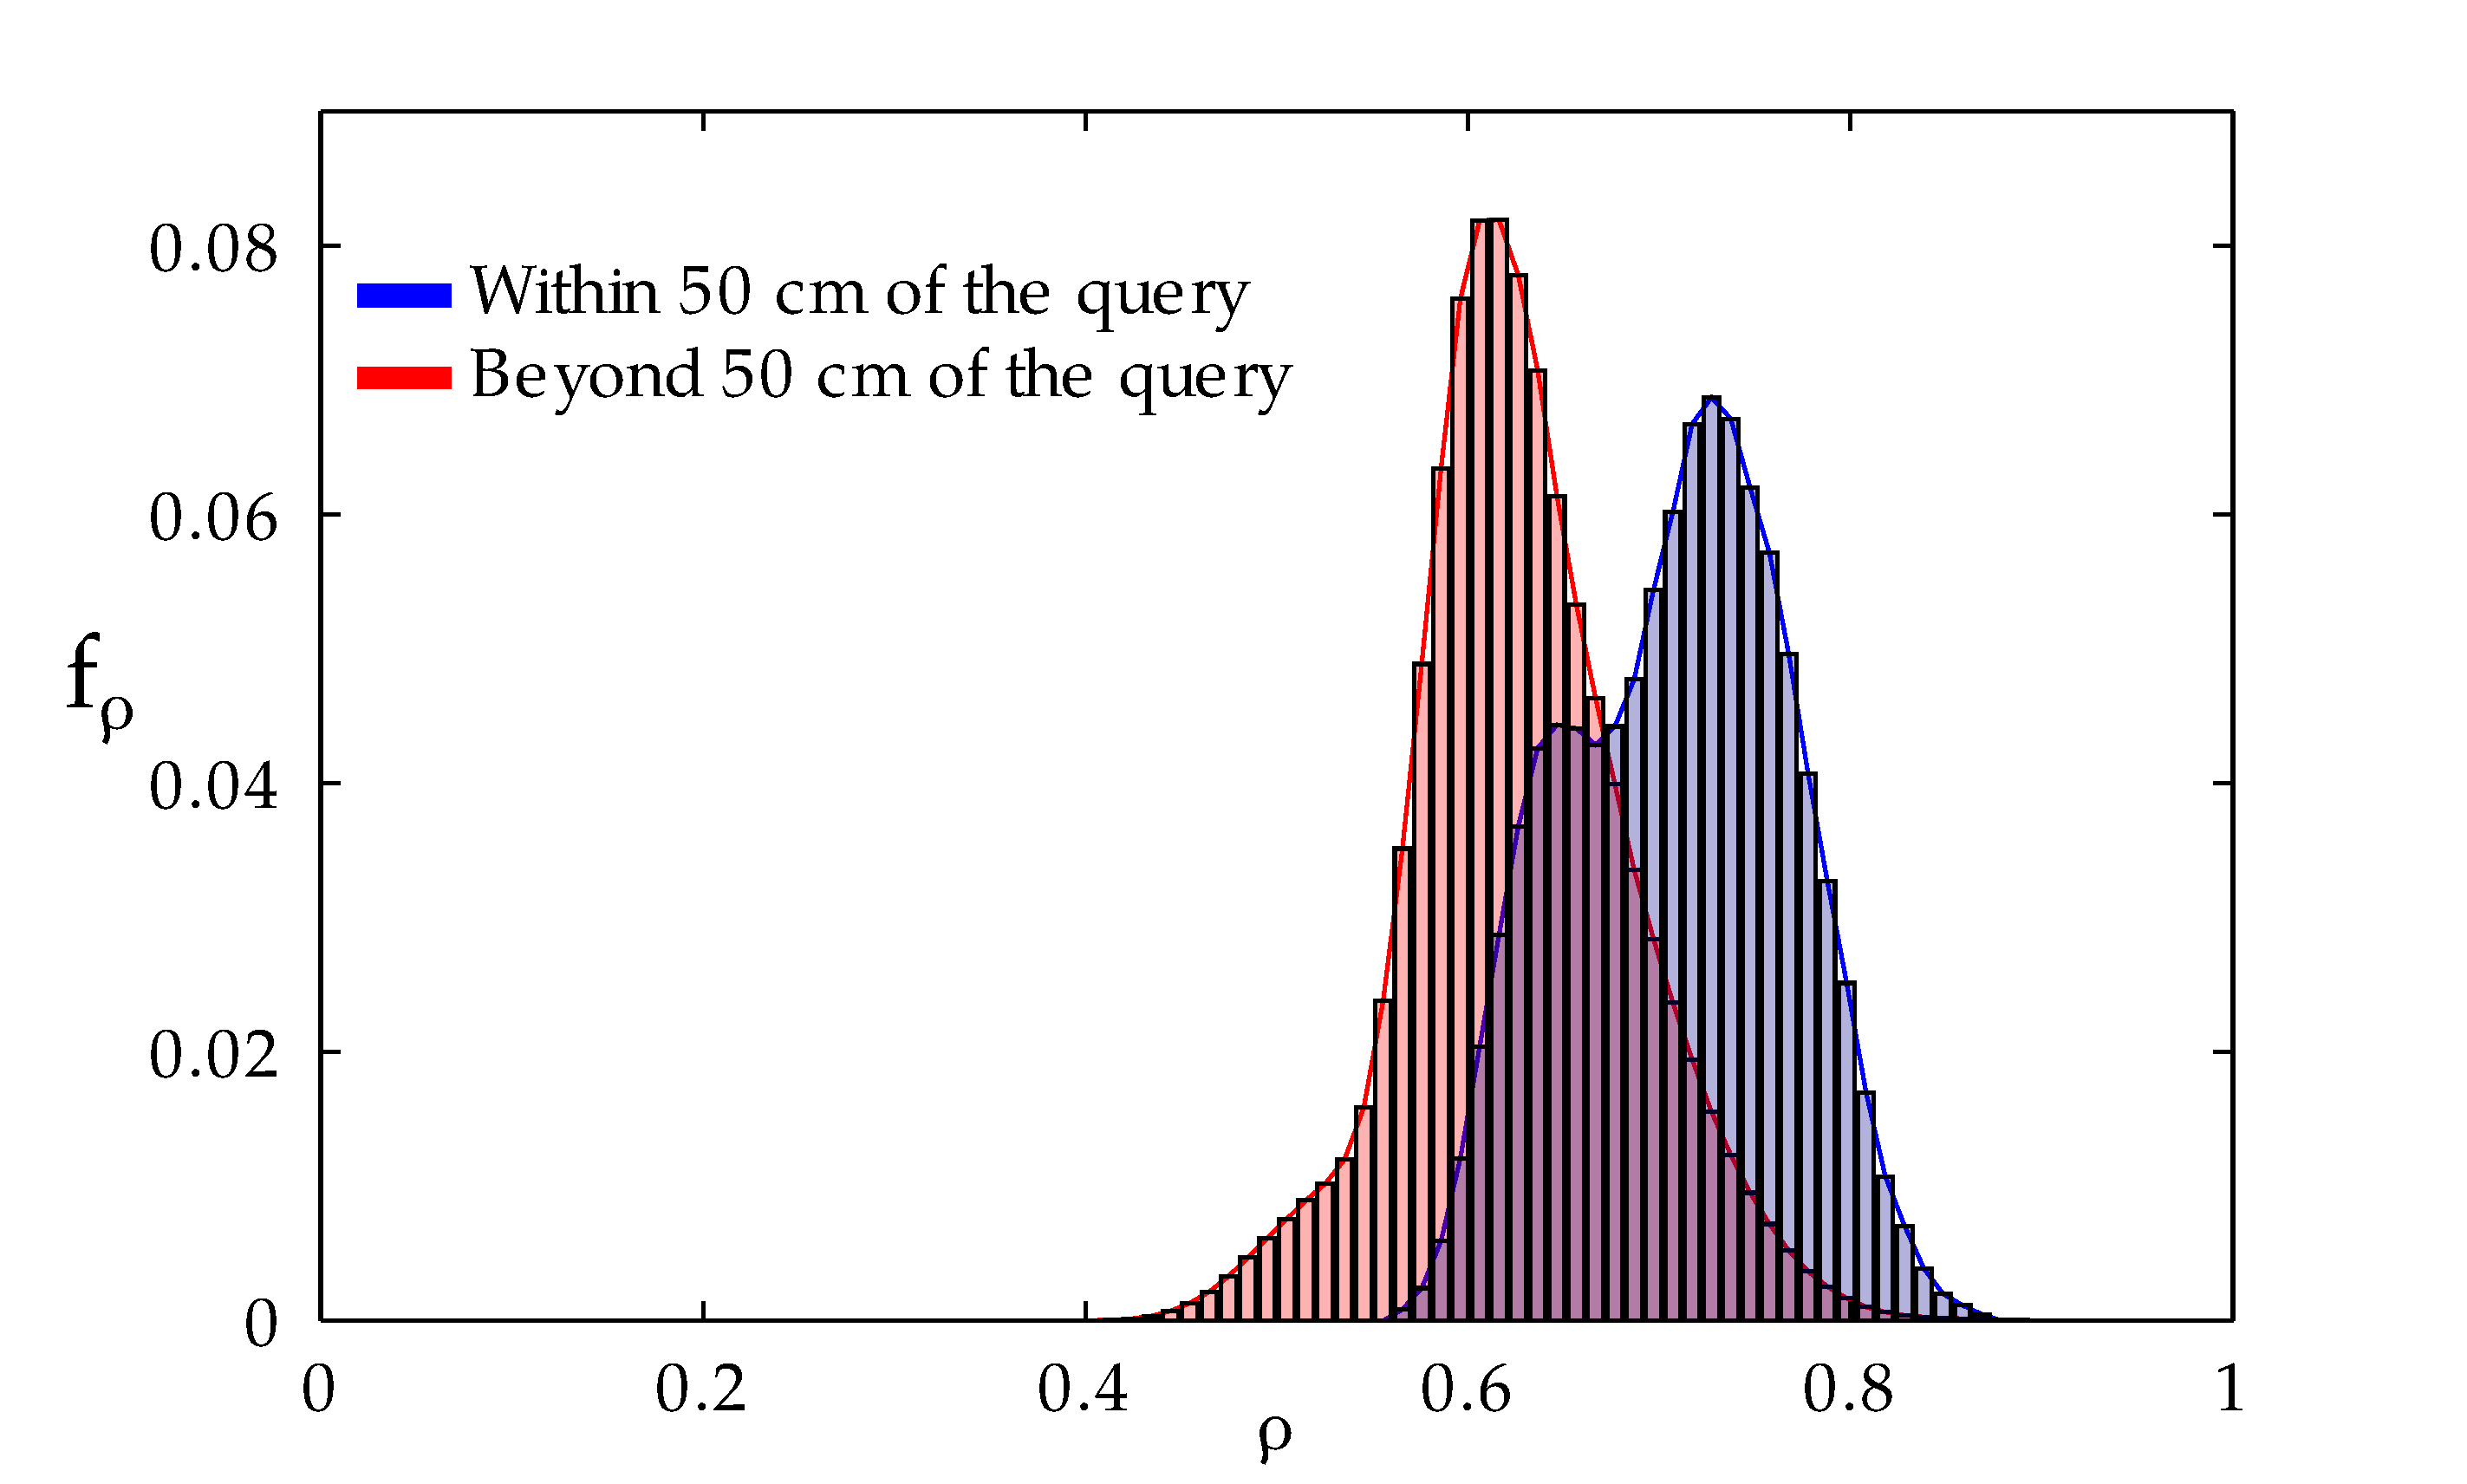
\includegraphics[width=\linewidth]{./gfx/Chapter02/C5distributions_no_smoothingWithSmoothedHistograms-latex.pdf}}
\caption{Tests of visual distinctiveness along paths: Distributions for the $\rho$ metric. Locations within a path, illustrating the distribution trends of the $\rho$-metric, all within a single 80 m path, but at different distances either within or outside 50 cm from known query submissions.}        
\label{fig:rhoDistribution}
\end{figure}

%%

%% WHAT AM I HOLDING?

\section{What Am I Holding?}

An increasing use for smartphones involves using \textit{visual search} in which a photograph taken with the phone is used as a query into a catalogue of database items.  Common items include paperbacks (books), compact-disc sleeves and art.  A closely related approach is the use of bar codes on items to look up both prices and more detailed product information.  

For the visually impaired, bar codes may be difficult to locate, and one would wish to allow recognition on objects and products from different points of view. The quality of a query image might also be below that of a sighted user.  For this reason, it is appropriate to assess the ability of visual search algorithms, designed for large-scale categorisation, to perform when the image queries are of low quality, as might occur in poor or variable lighting conditions.

The SHORT database~\cite{Rivera-Rubio2013a} provides such a dataset; and though it might consist of a small sub-sample of the categories in real-world product databases, it is  complementary and compliant with other datasets used in computer vision, such as the Pascal VOC database~\cite{everingham2010pascal} and ImageNet.  SHORT includes a query dataset acquired from 30 different smartphone cameras, with varying degrees of resolution, image quality and under two scenarios: sighted and blind-folded.  An example of typical queries is shown in Figure~\ref{fig:ShortQueries} below.

\begin{figure}
\centering
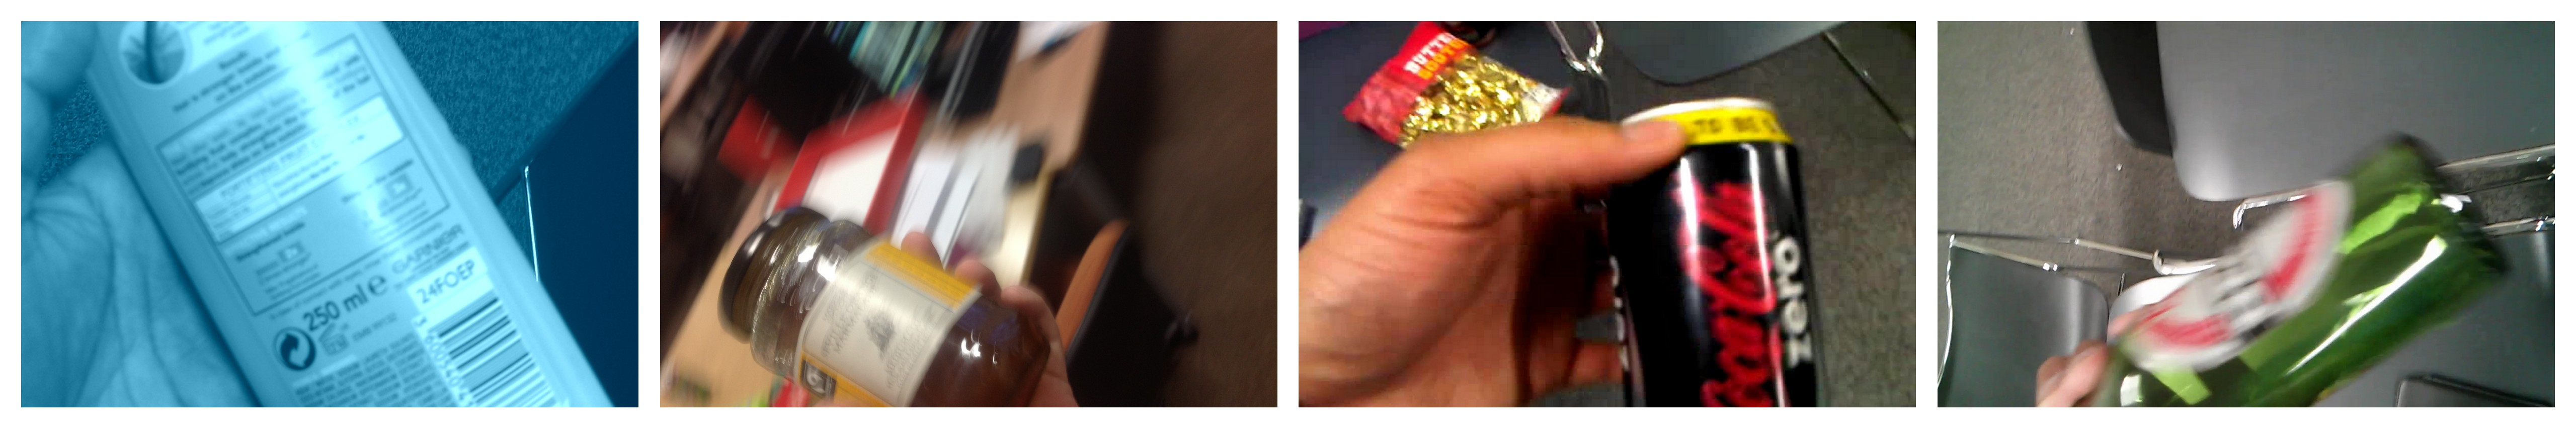
\includegraphics[width=\textwidth]{./gfx/Chapter02/TestDatasetCollage4imgs.jpg}
\caption{The SHORT database contains thousands of query images that form a representative set of examples of smartphone queries containing everyday household or packaged food products.}
\label{fig:ShortQueries}
\end{figure}

The dataset contains a mixture of stills and video clips, including nearly 135,000 video frames and more than 4,000 still images of 100 popular grocery items.  Image sizes range from under 100,000 pixels to over 6 megapixels. In Chapter \ref{ch:chapter3} a detailed description of the dataset and a complete evaluation will be provided.



\section{Initial experimental Results} \label{sec:expResults}

\subsection{Navigation}

I acquired a number of visual paths with a mobile phone (Nexus 4) in what was the pilot study for the RSM dataset (\url{http://rsm.bicv.org}) described in later chapters.  These visual paths take the form of video acquisitions, captured with the phone pointing in the direction of motion, and recording at 30 fps at 1920 $\times$ 1080 resolution. The images were then downsampled to a resolution of 192 $\times$ 108 pixels. The number of images captured along the paths raises the complexity of the image matching problem task: there are typically 2,000 images per path.

%For the analysis of the distribution of the scores $\gamma$ and $\rho$, as shown in Figure~\ref{fig:gammaDistribution} and \ref{fig:rhoDistribution}, VLFEAT's~\cite{Vedaldi2008} implementation of SIFT~\cite{lowe2004distinctive} descriptors has been used.

For the analysis of the distribution of the scores $\gamma$ and $\rho$, VLFEAT's~\cite{Vedaldi2008} implementation of SIFT~\cite{lowe2004distinctive} descriptors has been used.

\begin{figure}
\begin{center}
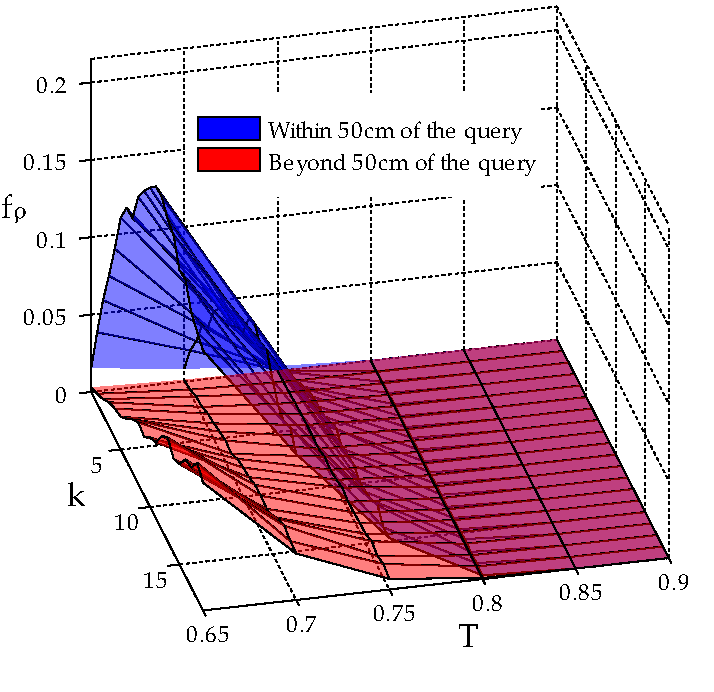
\includegraphics[width=.8\linewidth]{./gfx/Chapter02/C1twoTestWithBootstrapping2.pdf}
\caption{Fraction of values of $\rho$ exceeding a threshold $T$ in $k$ consecutive database frames.}
\label{fig:rocTwoParametersC5}
\end{center}
\end{figure}

The use of statistics randomly sampled with replacement, commonly called \textit{bootstrap} statistics, was appropriate for this study because, for example, in the navigational context, it allows sampling distributions of distances across the whole image database of around 400,000 possible pairings of visual path images.

In the case of the $\rho$ metric, these bootstrapped measurements have revealed the existence of visual distinctiveness between positions that are ``close'' or ``far'' along a path from a given query. In Figure~\ref{fig:rhoDistribution} I double-filtered the distribution of the $\rho$ values with a one-point moving average. This clearly shows that values of $\rho$ closer to one are useful for discriminating positions belonging to a specific visual path. These results have motivated the search for a threshold on the values of $\rho$ and the use of consecutive database frames to maximise discriminability, as illustrated in Figure~\ref{fig:rocTwoParametersC5}.


%%

%%  Discussion \& Conclusions

\section{Discussion \& Conclusions}

In this chapter I have presented the preliminary studies that laid the foundations for the work described in the remainder of this dissertation. The motivation was the same for both navigation and object recognition applications: mobile, appearance-based solutions with an emphasis in the assistive case. As we will see, the results presented in the following chapters are also applicable to sighted users. However, the design of the experiments always had the blind and partially sighted user in mind, as I believe that all serious design should be inclusive and therefore usable for both sighted and visually impaired. 

There are several conclusions to the pilot work reported here.  First, in the navigation context, there is an opportunity to use information from visual paths to provide an indication of which path a user might be on relative to previous journeys.  Although this study is limited to early findings with basic, standard techniques; it does indeed indicate that distinctive information can be harvested from visual paths with great ease.  For example, the resolutions of the images used in Section 2 contained only 1\% of the pixels in the captured images!  Yet, decisions on $\rho$ do seem to allow reasonably accurate estimates of where one is likely to be along a path, subject to appropriate verification being performed, perhaps using higher resolution images. With extra processing to perform geometric verification of match locations along the path, the idea of mapping images to a location looks quite feasible.

In the navigational context, the possibility of obscured views has not been considered, either during path collection or query collection. However, the density of the queries is also low relative to the number of queries that would normally be taken. For example, at a normal walking rate, one could easily collect more than 10 frames within 1 metre. Such an image sampling rate would give more opportunity to capture unobscured visual patches along a path. The caveat is that one would have to include modules for recognising obstructions or moving objects, such as people, within the frame, and remove query descriptors at  spatial scales that would include such regions. Since a key reason for incorporating computer vision into navigational aides would be to detect path obstructions and hazards, Chapter \ref{ch:chapter4} introduces a set of benchmarks using a collection of standard and custom ``dense'' descriptors that seem to be specially well-suited for this task.

In the context of hand-held objects from the SHORT database, a realistic database would be expected to have thousands of products. The category depth of SHORT is more appropriate to home use by a single user. I have presented the challenges of object recognition for the blind a partially sighted users and have introduced the SHORT database as a necessary benchmark for recognition algorithms that tackle hand-held, wearable and/or assistive applications. In Chapter \ref{ch:chapter3} I will evaluate the performance of baseline descriptor (SIFT) and bag-of-visual-words (BOVW) methods and establish retrieval comparisons that justify the need for a more challenging dataset that reflects hand-held and wearable vision.

%The retrieval mechanisms described here are not scalable: we did not use visual words in this study, although our tests are indicative of what one might apply in a post bag of visual words (BOVW) verification of rankings based on descriptor distances.

%Perhaps the most surprising factor of both of the feasibility studies reported here -- hand-held object recognition and the visual paths, is that the features used for both cases rely on the same set of tools: image descriptors that can be computed very quickly.  This is the subject for ongoing research in this area.


%*****************************************
%*****************************************
%*****************************************
%*****************************************
%*****************************************